\section{Numerical evidence and transportation interpretation}\label{sec:numerics}
Sioux Falls absolute accounts use benchmark flows in veh/h and time units of $0.01$ h; multiply an account by $0.01$ for the hourly vehicle-hour total. Anaheim uses vehicle-minutes per hour. All experiments use the stated fixed-path logit-SUE assignment models and prespecified demand scenarios; shares reported over boundary families are enumeration shares over those families. Table~\ref{tab:experimentmap} maps the five experiments; the section answers three questions in order: when one boundary summary is adequate, what generates spatial variation, and what a complete spatial profile with compact summaries looks like.
\begin{table}[pos=tb]
\caption{Experiment map.}\label{tab:experimentmap}
\begin{tabular*}{\tblwidth}{@{\extracolsep{\fill}}llll}
\toprule
Ex. & Network and queries & Purpose & Region families\\
\midrule
A & Sioux Falls, 8 largest ODs & background rerouting, spatial ranges & unrestricted, connected\\
B & Sioux Falls, 6 diverse ODs & signs, mechanisms, screenlines & connected, straight screenlines\\
C & Sioux Falls, 18 stratified ODs & common summaries, load levels, tolerance & fixed geometric family\\
D & Anaheim, 6 largest ODs & complete profiles, piecewise summaries & distance-progress family\\
E & learned models, 96 demand paths & explanation error, response supervision & geometric and full-boundary\\
\bottomrule\end{tabular*}\end{table}

\subsection{When is one boundary summary adequate?}\label{sec:adequate}
Sioux Falls has 24 nodes and 76 arcs in one cycle atom. Its structural weight condition is therefore the same for every OD; the experiments measure variation due to realized responses and heterogeneous marginal costs. The query-dependent classification is illustrated separately in Figure~\ref{fig:blockcut}.

Six input-selected queries away from node 10 change jointly from $0.2$ to $1.6$ times their base values with all other demands fixed and routes responsive; they are the shortest and longest free-flow ODs in each demand tercile (Appendix~\ref{supp:newod}). Table~\ref{tab:newod} reports their ranges. The two-stage rule of Section~\ref{sec:stability} separates them sharply: the geometric accounts for $(7,18)$ lie in $[642,702]$, their midpoint $672$ has maximum absolute error $30$, or $4.3\%$ of the largest account, and this family admits one common summary at a $5\%$ tolerance; the $(1,19)$ and $(7,12)$ geometric ranges cross zero and require boundary-specific reporting at every tolerance considered below.
\begin{table}[pos=htbp]
\caption{System contributions and spatial ranges for six prespecified queries,
setting C (TSTT units). Connected: all admissible connected regions;
screenline: the geometric family constructed independently of attribution
values. All $C_j$ are positive. Origin-cut accounts, negative shares, and
neighbourhood ranges are retained in Appendix~\ref{supp:newodaccuracy}.}
\label{tab:newod}
\small
\begin{tabular*}{\tblwidth}{@{\extracolsep{\fill}}lrrr}
\toprule
OD & $C_j$ & Connected [min, max] & Screenline [min, max]\\
\midrule
$(7,18)$ & $672.9$ & $[634{,}\ 710]$ & $[642{,}\ 702]$ \\
$(1,19)$ & $50{,}097.7$ & $[-13{,}502{,}\ 24{,}260]$ & $[-2{,}767{,}\ 22{,}124]$ \\
$(4,5)$ & $2{,}826.0$ & $[2{,}396{,}\ 3{,}452]$ & $[2{,}652{,}\ 3{,}176]$ \\
$(1,15)$ & $77{,}403.2$ & $[-8{,}286{,}\ 40{,}540]$ & $[511{,}\ 36{,}621]$ \\
$(6,8)$ & $73{,}964.9$ & $[35{,}307{,}\ 66{,}695]$ & $[45{,}230{,}\ 65{,}286]$ \\
$(7,12)$ & $117{,}482.3$ & $[-17{,}616{,}\ 60{,}029]$ & $[-2{,}967{,}\ 57{,}780]$ \\
\bottomrule
\end{tabular*}
\end{table}

Experiment C widens the view from six queries to an input-only selection of 18 of the 528 positive Sioux Falls OD demands, taking two lexicographically predetermined positions from each demand-by-free-flow-time tertile cell. Each OD changes alone over $\pm10\%$ and $\pm20\%$ intervals while other demands remain fixed with endogenous rerouting; the same 36-direction geometric family is used throughout, and Appendix~\ref{sec:coverage} reports every query and both widths. For each nonempty family, let $\beta=(\phi_{\max}+\phi_{\min})/2$ and $\varepsilon=(\phi_{\max}-\phi_{\min})/2$. This common summary minimizes the largest absolute discrepancy, so every reported boundary satisfies $|\phi(U)-\beta|\leq\varepsilon$. The reported normalized error is
\begin{equation}
r_j^{\mathcal F}=100\,\varepsilon_j^{\mathcal F}\Big/\max\bigl(|\phi_{j,\min}^{\mathcal F}|,|\phi_{j,\max}^{\mathcal F}|\bigr),
\label{eq:normerror}
\end{equation}
the absolute deviation of every account from the common value as a
percentage of the family's largest account magnitude; it does not bound
each account's own relative error. We apply a fixed descriptive tolerance
$r_j^{\mathcal F}\leq5\%$; this is a reporting choice rather than a
transport welfare threshold. When all accounts in a family share one
sign, $r_j^{\mathcal F}\leq50\%$, so values near $50\%$ indicate that
the smallest magnitude is far below the largest, not that the accounts
nearly agree.
At $\pm10\%$ and $\pm20\%$, respectively, 1 and 1 of 18 queries meet this tolerance, while 1 and 1 have accounts of both signs. The median geometric-to-unrestricted spread ratio is 0.574 at both widths.
\begin{table}[t]\centering\small\caption{Common-summary examples at $\pm20\%$. The four rows show the two smallest and two largest normalized summary errors among the fixed 18 queries. Normalized error is Eq.~\eqref{eq:normerror}; absolute values use the Sioux Falls cost units.}\label{tab:coverage_summary}\begin{tabular}{lrrrrrr}\toprule OD & System & Minimum & Maximum & $\beta$ & $\varepsilon$ & Norm.\ err.\ (\%)\\\midrule
(12,3) & 337.2 & 330.7 & 340.2 & 335.5 & 4.8 & 1.4\\
(4,3) & 507.2 & 429.0 & 535.0 & 482.0 & 53.0 & 9.9\\
(18,14) & 3422.3 & 150.8 & 1929.7 & 1040.2 & 889.5 & 46.1\\
(6,21) & 4577.8 & -3.4 & 2349.4 & 1173.0 & 1176.4 & 50.1\\
\bottomrule\end{tabular}\end{table}
\begin{figure}[t]\centering
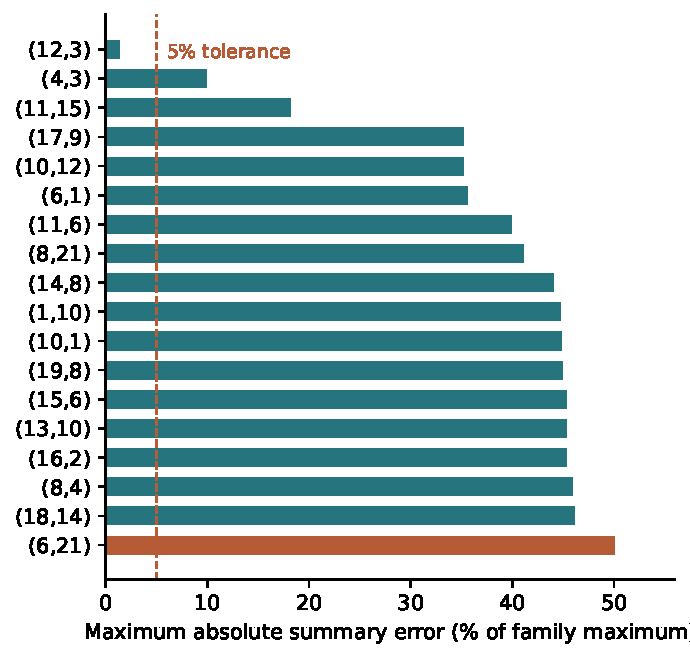
\includegraphics[width=0.97\linewidth]{../figures/fig_v106_summary_error_ranking.pdf}
\caption{Maximum absolute summary error, as a percentage of each
family's maximum account magnitude (Eq.~\eqref{eq:normerror}), over all
18 input-stratified queries at $\pm20\%$, with the queries reordered by
error. The tolerance is fixed at $5\%$; the complete account intervals
appear in Figure~\ref{fig:coverageintervals} in
Appendix~\ref{sec:coverage}.}\label{fig:commonsummary}\end{figure}

The $\pm10\%$ and $\pm20\%$ summaries of the same 18 queries are close in normalized terms, so further subdividing the perturbation width adds little information. The congestion state of the baseline is the more informative axis. All 528 demands are therefore scaled jointly to $0.7$, $1.0$ and $1.3$ times their published values; at each level the level equilibrium is solved once, the focal query alone moves by $\pm20\%$, other demands stay fixed with responsive routes, and the endpoint identity supplies the attribution column. The level-1.0 rows are the existing $\pm20\%$ results; levels $0.7$ and $1.3$ add 74 equilibrium solves under the identical geometric family and masks.
\begin{table}[t]\centering\small
\caption{Common-summary statistics across baseline load levels (18
queries, focal $\pm20\%$, same 36-direction family). Normalized error
is Eq.~\eqref{eq:normerror}; the ratio column is the median
geometric-to-unrestricted spread ratio.}\label{tab:loadlevels}
\begin{tabular}{rrrrrr}\toprule
Level & Queries within $5\%$ & Mixed signs & Median error (\%) & Median ratio & Max.\ negative share\\\midrule
$0.7$ & 2 & 0 & 34.5 & 0.529 & 0.000\\
$1.0$ & 1 & 1 & 44.4 & 0.574 & 0.0067\\
$1.3$ & 0 & 3 & 45.2 & 0.563 & 0.0403\\
\bottomrule\end{tabular}\end{table}
Table~\ref{tab:loadlevels} shows a monotone pattern: under the light
baseline, accounts are flatter across the family --- the median
normalized error falls to $34.5\%$, two queries satisfy the $5\%$
tolerance and no family crosses zero --- whereas the heavy baseline
makes every query exceed the tolerance, three families mix signs and
the negative share of $(6,21)$ reaches $4\%$. Per-query normalized
errors rise from the light to the heavy level for 17 of 18 queries
(e.g.\ $(10,12)$: $18.6\to35.2\to40.3$; $(1,10)$: $31.2\to44.8\to48.0$).
Across the load levels, light-load conditions admit transferable single
summaries more often, and heavy-load conditions require
boundary-specific reporting.

The dependence on the reporting tolerance itself is summarized by the
frontier of Table~\ref{tab:tolerance}. Relaxing the tolerance from
$2.5\%$ to $10\%$ keeps the number of Sioux Falls queries admitting a
single common value between zero and two at every load level (rising
by at most one per level), while the median number of contiguous
segments per query falls from 42--53
to 18--22 of a median 86.5 family regions; on Anaheim's ordered
families the same relaxation raises the compression of the 83--211
accounts per query from $91.4\%$ (6--21 segments) to $96.4\%$
(3--12 segments). With the same segment count, equal-count partitions
have median worst-segment error $2.7$--$10.4$ times the tolerance on
Sioux Falls and $4.7$--$18.8$ times on Anaheim, so position-aware
segmentation is what buys the error control, not the segment count
alone.
\begin{table}[t]\centering\small
\caption{Tolerance sensitivity of common summaries (experiment C for
Sioux Falls, 18 queries per level; experiment D for Anaheim, six
queries). Single: number of queries whose family admits one common
value at the stated tolerance; segments: median (Sioux Falls, of a
median 86.5 regions) or per-query range (Anaheim) of minimal contiguous
segments; compression: $1-$segments/regions.}\label{tab:tolerance}
\begin{tabular}{rrrrr}\toprule
Tolerance $\tau$ & Sioux single ($0.7/1.0/1.3$) & Sioux med.\ segments & Anaheim segments & Anaheim compression\\\midrule
$2.5\%$ & $2/1/0$ & $42.0/50.5/52.5$ & $6$--$21$ & $91.4\%$\\
$5\%$ & $2/1/0$ & $29.5/38.0/38.5$ & $4$--$14$ & $93.8\%$\\
$7.5\%$ & $2/1/1$ & $22.5/26.5/29.0$ & $3$--$12$ & $95.5\%$\\
$10\%$ & $2/2/1$ & $18.0/21.0/22.0$ & $3$--$12$ & $96.4\%$\\
\bottomrule\end{tabular}\end{table}

The load-level trend has a theory-side counterpart in the node
representation. For each of the 18 columns and three levels, the
imbalance vector $d_j$ of Eq.~\eqref{eq:endpointd} has norm
$\norm{d_j}_2$ rising from a median of $1196.4$ at level $0.7$ to
$4803.2$ at $1.0$ and $15763.3$ at $1.3$ --- a $13.2$-fold increase
from the light to the heavy baseline --- while the unrestricted range
$S_j$ rises from $3102.2$ to $52766.2$. Across all 54 query--level
pairs, the rank correlation between $\norm{d_j}_2$ and the
geometric-family spread is $0.99$ (Spearman; $0.99$ for $S_j$), and the
realized ratio $S_j/\norm{d_j}_2$ has median $2.53$ against the
Cauchy--Schwarz bound $\sqrt{n-2}=4.69$ of Eq.~\eqref{eq:rangebound}.
The normalized summary error, whose denominator varies by query,
correlates more moderately ($0.53$). The theory thus not only classifies
when spatial ranges vanish; the load-level growth of the ranges is
consistent with heavier congestion weighting amplifying the node
imbalance that Eq.~\eqref{eq:cutspread} sums into the spatial range ---
a mechanistic reading, since the load levels change the realized
weights, responses and demand increments together rather than the
weights alone.

\subsection{What generates spatial variation?}\label{sec:variation}
Experiment A varies the background treatment. Eight largest published OD demands, all incident to node 10, change jointly from $0.2$ to $1.6$ times their base values; every study OD has ten fixed paths. Settings A, B and C use zero background, frozen background link flows and fixed background demands with endogenous rerouting, respectively. Setting C assigns all 528 positive demands (full protocols in Appendix~\ref{supp:fields}).
Uniform weights provide a compatible control. The active-link outcome $T(F)=F_{10\to16}$ preserves the $(10,16)$ direction but permits a response-dependent scale; TSTT produces internal imbalance. Figure~\ref{fig:respfield} illustrates these patterns. For its seed-zero TSTT response, expanding $\{10\}$ to $\{10,17\}$ lowers the account from $5.77\times10^4$ to $4.34\times10^4$, approximately $92\%$ of the unrestricted spread. The direct-SUE decrease is $24.80\%$ of its own origin-cut account (Appendix~\ref{supp:accuracy}). Both sides of these regions are connected. Free-flow weights explain $84.7\%$ of the node-17 imbalance: all incident links have free-flow time 2 except $10\leftrightarrow17$ with time 8, giving $[B\operatorname{diag}(t_0)G_j]_{17}=6(G_{10\to17,j}-G_{17\to10,j})$.

Table~\ref{tab:cutspreadperod} shows three representative queries of the eight under the three background settings (the complete table is in Appendix~\ref{supp:additional}); rerouting produces appreciable spatial variation for every query, and connected regions retain $60.41$--$76.85\%$ of the unrestricted range across the full set. Normalizations use each setting's own origin account: for $(17,10)$, the percentage falls from $59.95\%$ in A to $54.77\%$ in C while the absolute spread rises from 17,607.8 to 123,202.1, approximately sevenfold.
\begin{table}[pos=htbp]
\caption{TSTT cut ranges as percentages of each account's absolute
origin-cut value; three representative queries shown, complete table in
Appendix~\ref{supp:additional}. A: zero background; B: frozen background
flows; C: background demands fixed, all traffic re-equilibrated. Learned
values are five-seed medians (ranges); all SUE columns are direct
($41$ quadrature points, implicit sensitivities).}\label{tab:cutspreadperod}
\small
\begin{tabular*}{\tblwidth}{@{\extracolsep{\fill}}lccccc}
\toprule
& \multicolumn{4}{c}{Unrestricted range (\%)} & Connected (\%)\\
\cmidrule(lr){2-5}\cmidrule(lr){6-6}
OD & Learned A & SUE A & SUE B & SUE C & SUE C\\
\midrule
$(17,10)$ & $59.71$ $(58.92$--$61.23)$ & $59.95$ & $56.38$ & $54.77$ & $35.27$ \\
$(16,10)$ & $36.80$ $(36.41$--$38.40)$ & $36.86$ & $39.99$ & $166.26$ & $127.72$ \\
$(11,10)$ & $0.18$ $(0.03$--$0.27)$ & $0.0073$ & $0.79$ & $81.09$ & $48.98$ \\
\bottomrule
\end{tabular*}
\end{table}
\paragraph{Same-state response decomposition.}\label{subsec:bgsplit}
Comparing A, B and C changes both costs and sensitivities. At each common setting-C state, split responses into study and background parts, with $BJ_j^{\mathrm{study}}=\mu_j$ and $BJ_j^{\mathrm{bg}}=0$. Weight both by the same total-flow TSTT gradient, yielding
\begin{equation}
\widetilde C_j^{\mathrm{tot}}=\widetilde C_j^{\mathrm{study}}+\widetilde C_j^{\mathrm{bg}}.
\label{eq:bg_attribution}
\end{equation}
At node 15 for $(10,16)$, study and background divergence contributions are $-973.1$ and $49{,}103.4$. Yet on the specified expansion $\{10\}\to\{10,17\}$, the account changes only $-3361.1$ ($-1305.0$ study, $-2056.1$ background), or $1.23\%$ of the initial account. Large extremal variation can coexist with similar selected accounts. Component differences add at a fixed region pair; their separate ranges do not add in general.

\paragraph{Free-flow and congestion mechanisms.}\label{subsec:newod}
For BPR costs, $g_e'=t_{0,e}+0.75t_{0,e}(F_e/c_e)^4$. Crossing these two weight terms with the two response terms gives four additive contributions, evaluated at identical states and the same reported boundary:
\[
\phi_j(U_-)=\sum_{a\in\{\mathrm{ff,cong}\}}\sum_{b\in\{\mathrm{study,bg}\}}\phi_j^{a,b},
\qquad \phi_j^{a,b}=-\Delta q_j\int_0^1\mathbf1_{U_-}^{\top}BD_\lambda^aJ_j^b(\lambda)\,d\lambda.
\]
Table~\ref{tab:ffcong} distinguishes the mechanisms behind the sign-crossing queries of Table~\ref{tab:newod}: study congestion dominates $(1,19)$, both congestion terms are negative for $(1,15)$, and background congestion dominates $(7,12)$. The combined free-flow contribution stays positive. The decomposition is additive at a common equilibrium state and identifies the contribution of each response--weight component.
\begin{table}[pos=htbp]
\caption{Four parts of the same boundary account at the reported
$U_-$ (setting C, six-query protocol; TSTT units; identical $41$-point
states, responses, and boundaries as Table~\ref{tab:newod}). Study
includes all six query ODs; background includes the other $522$.
Columns cross free-flow/congestion weights with study/background
responses. Entries are rounded independently.}\label{tab:ffcong}
\small
\begin{tabular*}{\tblwidth}{@{\extracolsep{\fill}}lrrrrr}
\toprule
OD & Free-flow study & Free-flow background & Congestion study & Congestion background & Total\\
\midrule
$(1,19)$ & $-361.3$ & $+759.0$ & $-17{,}357.9$ & $+3{,}458.6$ & $-13{,}501.6$ \\
$(1,15)$ & $+1{,}541.8$ & $+333.8$ & $-6{,}537.4$ & $-3{,}624.2$ & $-8{,}286.0$ \\
$(7,12)$ & $+3{,}897.0$ & $-1{,}311.1$ & $+125.5$ & $-20{,}327.6$ & $-17{,}616.2$ \\
\bottomrule
\end{tabular*}
\end{table}
The sign pattern itself is a spatial property, not a magnitude artefact. Negative accounts occupy $17.8\%$, $2.5\%$ and $7.3\%$ of the 14,477, 15,191 and 16,943 connected regions of the three sign-crossing queries. For $(1,19)$, the connected minimum $-13{,}501.6$ is attained on a 13-node region, whereas a 13-node free-flow neighbourhood has account $+10{,}756.0$: region size alone does not determine the account. At the minimizing boundary, outgoing attributions sum to $7{,}867.3$ and incoming attributions to $21{,}368.8$, so the signed crossing-link account is negative while $C_j=50{,}097.7>0$; Figure~\ref{fig:negmech} maps all 26 crossing links. Figure~\ref{fig:screenlines} shows the same contrast on two straight screenlines of the prespecified geometric family: the minimum and maximum screenline accounts of $(1,19)$ have opposite signs under one positive network-wide contribution.
\begin{figure}[pos=tb]
\centering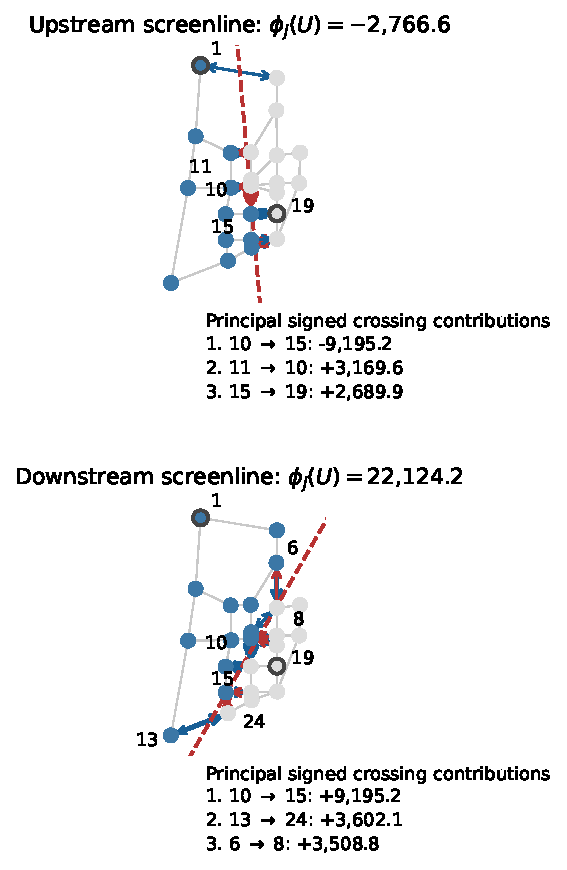
\includegraphics[width=0.64\linewidth]{../figures/fig_screenlines_v106.pdf}
\caption{Contrasting screenline accounts for the same positive OD
contribution. Two straight screenlines for OD $(1,19)$, setting C. Blue
nodes belong to $U$; grey nodes are outside; dashed lines separate the
two sides. Node $1$ is inside and node $19$ outside in both panels.
Upstream/downstream names the position of the separating line along the
corridor: its crossing progress with the straight origin--destination
segment is $0.61$ (upper) versus $0.78$ (lower). The two accounts have
opposite signs while the network-wide contribution is positive. The
lines are the minimum and maximum of the prespecified geometric family;
the complete irregular connected minimum and its crossing-link
decomposition appear in Figure~\ref{fig:negmech}.}
\label{fig:screenlines}\end{figure}
The straight-screenline family uses 36 directions at $5^\circ$ intervals, gaps between node projections, two-sided connectivity and duplicate removal; construction is independent of attribution. It contains 23--152 distinct regions per query. The $(1,19)$ and $(7,12)$ negative minima occur on 2/152 and 10/148 screenlines. Origin-centred hop and free-flow neighbourhoods remain positive but can differ in magnitude by factors 8.9, 9.0 and 3.4 for the three sign-crossing queries (Appendix~\ref{supp:newodaccuracy}). Sign stability and common-value accuracy are distinct properties.
